\documentclass[tikz,border=2pt]{standalone}
\usepackage{amsmath}
\usetikzlibrary{arrows.meta}
\begin{document}
% Matching Pennies as a tree: if player 2 does not observe player 1, her two nodes form one
% information set h_2 (2 strategies); if she observes, they are two singletons (2*2 = 4 strategies).
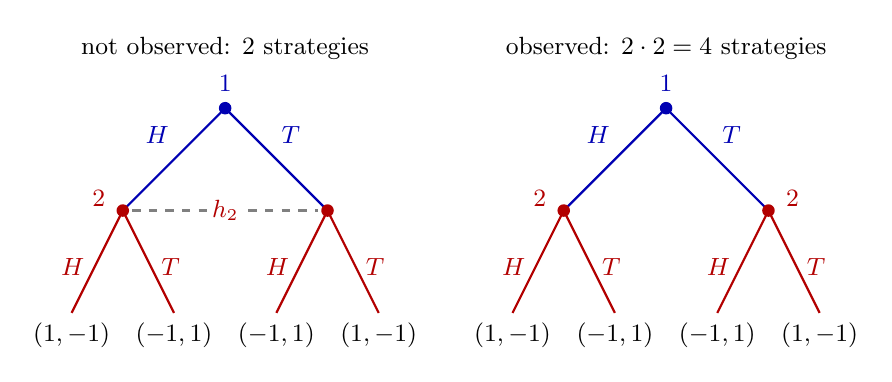
\begin{tikzpicture}[font=\small, >={Latex[length=2mm]},
    dec/.style={circle, fill, inner sep=1.6pt}]
  \foreach \ox/\obs in {0/0, 5.6/1} {
    \begin{scope}[xshift=\ox cm]
      % edges
      \draw[thick, blue!70!black] (1.95,0) -- node[above left, pos=0.45] {$H$} (0.65,-1.3);
      \draw[thick, blue!70!black] (1.95,0) -- node[above right, pos=0.45] {$T$} (3.25,-1.3);
      \draw[thick, red!70!black] (0.65,-1.3) -- node[left, pos=0.55] {$H$} (0,-2.6);
      \draw[thick, red!70!black] (0.65,-1.3) -- node[right, pos=0.55] {$T$} (1.3,-2.6);
      \draw[thick, red!70!black] (3.25,-1.3) -- node[left, pos=0.55] {$H$} (2.6,-2.6);
      \draw[thick, red!70!black] (3.25,-1.3) -- node[right, pos=0.55] {$T$} (3.9,-2.6);
      % nodes
      \node[dec, blue!70!black, label={[blue!70!black]above:$1$}] at (1.95,0) {};
      \node[dec, red!70!black] (a) at (0.65,-1.3) {};
      \node[dec, red!70!black] (b) at (3.25,-1.3) {};
      % leaves
      \foreach \x/\p in {0/{(1,-1)}, 1.3/{(-1,1)}, 2.6/{(-1,1)}, 3.9/{(1,-1)}}
        \node[anchor=north, inner sep=2pt] at (\x,-2.65) {$\p$};
    \end{scope}
  }
  % left: one information set
  \draw[dashed, thick, gray] (0.77,-1.3) -- (3.13,-1.3);
  \node[red!70!black, fill=white, inner sep=1pt] at (1.95,-1.3) {$h_2$};
  \node[red!70!black, anchor=east] at (0.55,-1.15) {$2$};
  % right: two singletons
  \node[red!70!black, anchor=east] at (6.15,-1.15) {$2$};
  \node[red!70!black, anchor=west] at (8.95,-1.15) {$2$};
  % captions
  \node[anchor=south] at (1.95,0.5) {not observed: $2$ strategies};
  \node[anchor=south] at (7.55,0.5) {observed: $2\cdot 2=4$ strategies};
\end{tikzpicture}
\end{document}
